\documentclass[UTF8,hyperref]{pkuthss}

%%%%%%%%%%%%%%%%%%%%%%%%%%%%%%%%%%%%%%%%%
% Article Notes
% Structure Specification File
% Version 1.0 (1/10/15)
%
% This file has been downloaded from:
% http://www.LaTeXTemplates.com
%
% Authors:
% Vel (vel@latextemplates.com)
% Christopher Eliot (christopher.eliot@hofstra.edu)
% Anthony Dardis (anthony.dardis@hofstra.edu)
%
% License:
% CC BY-NC-SA 3.0 (http://creativecommons.org/licenses/by-nc-sa/3.0/)
%
%%%%%%%%%%%%%%%%%%%%%%%%%%%%%%%%%%%%%%%%%

%----------------------------------------------------------------------------------------
%	REQUIRED PACKAGES
%----------------------------------------------------------------------------------------

\usepackage[T1]{fontenc} % For international characters
\usepackage{XCharter} % XCharter as the main font

\usepackage{natbib} % Use natbib to manage the reference
\bibliographystyle{apalike} % Citation style

\usepackage[english]{babel} % Use english by default

%----------------------------------------------------------------------------------------
%	CUSTOM COMMANDS
%----------------------------------------------------------------------------------------

\newcommand{\articletitle}[1]{\renewcommand{\articletitle}{#1}} % Define a command for storing the article title
\newcommand{\articlecitation}[1]{\renewcommand{\articlecitation}{#1}} % Define a command for storing the article citation
\newcommand{\doctitle}{\articlecitation\ --- ``\articletitle''} % Define a command to store the article information as it will appear in the title and header

\newcommand{\datenotesstarted}[1]{\renewcommand{\datenotesstarted}{#1}} % Define a command to store the date when notes were first made
\newcommand{\docdate}[1]{\renewcommand{\docdate}{#1}} % Define a command to store the date line in the title

\newcommand{\docauthor}[1]{\renewcommand{\docauthor}{#1}} % Define a command for storing the article notes author

% Define a command for the structure of the document title
\newcommand{\printtitle}{
\begin{center}
\textbf{\Large{\doctitle}}

\docdate

\docauthor
\end{center}
}

%----------------------------------------------------------------------------------------
%	STRUCTURE MODIFICATIONS
%----------------------------------------------------------------------------------------

\setlength{\parskip}{3pt} % Slightly increase spacing between paragraphs

% Uncomment to center section titles
%\usepackage{sectsty}
%\sectionfont{\centering}

% Uncomment for Roman numerals for section numbers
%\renewcommand\thesection{\Roman{section}}
 % Input the file specifying the document layout and structure

%----------------------------------------------------------------------------------------
%	ARTICLE INFORMATION
%----------------------------------------------------------------------------------------

\articletitle{笔记} % The title of the article
%SB\articlecitation{\cite{dubner1999assessing}} % The BibTeX citation key from your bibliography

\datenotesstarted{April 30, 2017} % The date when these notes were first made
\docdate{\datenotesstarted; rev. \today} % The date when the notes were lasted updated (automatically the current date)

\docauthor{Qian Wang} % Your name

%----------------------------------------------------------------------------------------
\usepackage{bm}
\usepackage{caption}
\usepackage{preview}
\usepackage{mathtools}
\usepackage{latexsym}
\usepackage{standalone}
\usepackage{wasysym}
% 提供 verbatiminput 命令和 comment 环境。
\usepackage{verbatim}
\usepackage{graphicx} % 图形包
\usepackage{datetime}
\usepackage{advdate}
\usepackage[top=1in, bottom=1in, left=1.25in, right = 1.25in]{geometry}
\usepackage{booktabs} % Allows the use of \toprule, \midrule and
\usepackage{latexsym}
\usepackage{amsmath,amssymb}
\usepackage{algorithm}
\usepackage{amsthm}
\usepackage[UTF8]{ctex}
\usepackage{listings}
\usepackage{color}
\usepackage{xcolor}
\usepackage{float}
\lstset{
	language=Python,
    numbers=left, 
    numberstyle= \tiny, 
    keywordstyle= \color{ blue!70},
    commentstyle= \color{red!50!green!50!blue!50}, 
    frame=shadowbox, % 阴影效果
    rulesepcolor= \color{ red!20!green!20!blue!20} ,
    escapeinside=``, % 英文分号中可写入中文
    xleftmargin=2em,xrightmargin=2em, aboveskip=1em,
    framexleftmargin=2em
}
\usepackage{anysize}
\marginsize{2cm}{2cm}{0cm}{2cm}

\begin{document}

\pagestyle{myheadings} % Use custom headers
%\markright{\doctitle} % Place the article information into the header

%----------------------------------------------------------------------------------------
%	PRINT ARTICLE INFORMATION
%----------------------------------------------------------------------------------------

\thispagestyle{plain} % Plain formatting on the first page

\printtitle % Print the title
%---------------------------------------------------------------------------------------
%	ARTICLE NOTES
%----------------------------------------------------------------------------------------

\cleardoublepage 
%\numberwithin{equation}{section}   公式按章 节 编号
\renewcommand{\theequation}{\arabic{section}.\arabic{equation}}
\cleardoublepage 
\chapter{Adaboost}

\section*{Introduction}
	本章内容来自于网络以及张志华老师的就《机器学习导论》课程

	本章基本内容就是给定一堆弱分类器,然后通过各种组合组成一个人强的分类器

\section{离散的Adaboost}

	离散的AdaBoost算法步骤:\boldmath  %公式加粗

	$w$表示给数据的权值,$\alpha$表示给分类器的权值

	\begin{enumerate}		
		\item start with weights $w_i = \frac{1}{N} \quad i=1...N$
		\item repeat for m=1 to M
			\begin{itemize}
				\item 使用输入数据训练一个分类器$G_m(x) \in (-1,1)$
				\item 计算误差err:
					\begin{equation*}
						E_w[I_(y_i\not \equiv G_m(x_i))]=\frac{\sum_{i=1}^{N}w_i I_(y_i\not \equiv G_m(x_i))}{\sum_{i=1}^{N}w_i}
					\end{equation*}
				\item 输出$\alpha_m = \frac{1}{2}log(\frac{1-err}{err})$,从这里可以看出分类器的误差越大,权值越小
				\item set $w_i = \frac{w_i}{Z_m} \exp(\alpha_m I_(y\not \equiv G_m(x))$,其中$Z_m$是规范化因子,\newline
				$Z_m=\sum_{i=1}^{N}w_i \exp(-\alpha_m y_i G_m(x_i))$如果一个数据点分类错了,那么给这个点的权值大一点。
			\end{itemize}
		\item 这样我们就得到了$G(x)=sign[\sum_{m=1}^{M}\alpha_m G_m(x)]$
	\end{enumerate}



%--------------------------------------------------------------------------------
%--------------------------------------------------------------------------------
%--------------------------------------------------------------------------------

\section{Forward Stagest Additive Modeling}

	考虑加法模型(additive model)\boldmath
	\begin{equation}
		f(x)=\sum_{m=1}^{M}\beta_{m}b(x;\gamma_{m})
	\end{equation}
	其中,$b(x;\gamma_{m})$为基函数,$\gamma_m$为基函数的参数,$\beta_m$为基函数的系数。

	在给定训练数据以及Loss Function的情况下,相当于一个加法模型$f(x)$相当于一个minimize Loss Function的问题:
	\begin{equation}
		min_{\beta_m,\gamma_m} \sum_{i=1}^{N}L(y_i,\sum_{m=1}^{M}\beta_{m}b(x;\gamma_{m}))
	\end{equation}
	从前向后,每一步值学习一个基函数及其系数,即每一步只需优化如下的损失函数:
	\begin{equation}
		min_{\beta,\gamma} \sum_{i=1}^{N}L(y_i,\sum_{m=1}^{M}\beta b(x;\gamma))
	\end{equation}
	\newline
	\newline

	前向分布算法:

	输入:训练数据$T={(x_1,y_1),...(x_N,y_N)}$,Loss Function$L(x,f(x))$,基函数$b(x;\gamma)$

	输出:加法模型$f(x)$

	\begin{enumerate}		
		\item 初始化$f_0(x)=0$
		\item repeat for m=1 to M
			\begin{itemize}
				\item 计算参数$\beta_m,\gamma_m$
				\begin{equation}
					(\beta_m,\gamma_m)=\arg\min_{\beta,\gamma} \sum_{i=1}^{N}L(y_i,f_{m-1}(x_i)\beta b(x;\gamma))
				\end{equation}
				\item 更新$f_m(x)=f_{m-1}(x)+\beta_m b(x;\gamma_m)$
			\end{itemize}
		\item 得到加法模型
				\begin{equation}
					f(x)=\sum_{m=1}^{M} \beta_m b(x;\gamma_m)
				\end{equation}
	\end{enumerate}
\cleardoublepage 
\chapter{Logistic Regression}

\section*{Introduction}
	本章内容主要来自于个人YY

\section{Sigmoid函数}
	\boldmath  %公式加粗
	sigmoid 函数的主要公式如下所示:
	
	\begin{equation}
		p(x) = \frac{1}{1+e^{-x}}
	\end{equation}		
	
	该公式主要用在二分类的问题中作为最后的预测结果分类,或者作为激活函数在神经网络中使用。
	
	为什么要使用sigmoid?暂时不清楚
	

\section{Logistic Regression}
	\boldmath  %公式加粗
	逻辑回归主要用在二分类问题中,最后给出该样本属于正类或者负类的概率,公式如下所示:
	
	\begin{equation}
		J(\theta) = - \frac{1}{m} \left[ \sum_{i=1}^{m} y^{(i)} log h_\theta(x^{(i)})+ (1-y^{(i)})log(1-h_\theta(x^{(i)})) \right]	
	
	\end{equation}
	
	通俗的来说,LR就是用来将两堆数据分来
	
	LR优点:
	
	\begin{itemize}
		\item 预测结果是介于0和1之间的概率
		\item 容易使用和解释
		\item 预测速度较快,计算量小
	\end{itemize}
	
	缺点:
	\begin{itemize}
		\item 当特征空间很大时,LR的性能不是很好,不能处理大量的特征
		\item 容易欠拟合
		\item 不能处理线性不可分的数据
		\item 对于非线性特征,需要进行转换
	\end{itemize}










	% \begin{enumerate}		
	% 	\item start with weights $w_i = \frac{1}{N} \quad i=1...N$
	% 	\item repeat for m=1 to M
	% 		\begin{itemize}
	% 			\item 使用输入数据训练一个分类器$G_m(x) \in (-1,1)$
	% 			\item 计算误差err:
	% 				\begin{equation*}
	% 					E_w[I_(y_i\not \equiv G_m(x_i))]=\frac{\sum_{i=1}^{N}w_i I_(y_i\not \equiv G_m(x_i))}{\sum_{i=1}^{N}w_i}
	% 				\end{equation*}
	% 			\item 输出$\alpha_m = \frac{1}{2}log(\frac{1-err}{err})$,从这里可以看出分类器的误差越大,权值越小
	% 			\item set $w_i = \frac{w_i}{Z_m} \exp(\alpha_m I_(y\not \equiv G_m(x))$,其中$Z_m$是规范化因子,\newline
	% 			$Z_m=\sum_{i=1}^{N}w_i \exp(-\alpha_m y_i G_m(x_i))$如果一个数据点分类错了,那么给这个点的权值大一点。
	% 		\end{itemize}
	% 	\item 这样我们就得到了$G(x)=sign[\sum_{m=1}^{M}\alpha_m G_m(x)]$
	% \end{enumerate}



%--------------------------------------------------------------------------------
%--------------------------------------------------------------------------------
%--------------------------------------------------------------------------------
\cleardoublepage 
\chapter{正则化方法}

\section*{Introduction}
	本章节内容主要介绍机器学习、深度学习总的正则化方法
	
	一般来说,所有的监督学习都可以最小化下面的函数来表示:
	
	\begin{equation}
		w = \arg \min_{w} \sum_{i}L(y_i,f(x_i;w)) + \lambda \Omega(w)
	\end{equation}
	
	其中,第一项一般为模型预测的结果与真实的结果之间的差距,可以用各种各样不同的函数来表示,第二项一般为正则化项,主要目的是使我们的模型更加简单,防止过拟合。

\section{L1 L2}
	\boldmath  %公式加粗
	
	\subsection{ill-condition}
	我们都知道优化问题有两大难题。一个是局部最小值的问题:我们要找的是全局最小值,如果局部最小值太多,那我们的优化算法就很容易陷入局部最小而不能自拔。另外一个就是ill-condition的问题。加入我们有个方程组$Ax=b$,我们要做的是求解$x$,如果$A$或者$b$稍微的改变,会使得$x$发生很大的变化,那么这个方程组系统就是ill-condition的,反之就是well-condition的。
	
	\begin{figure}[htbp]
	\centering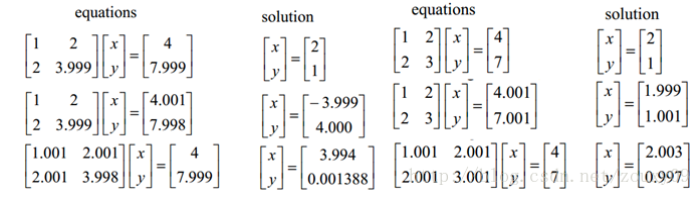
\includegraphics[width=6in]{img/3-1.png}
	\caption{ill-condition}\label{fig:3-1}
	\end{figure}
	
	第一行我们假设$Ax=b$,第二行我们稍微改变下$A$,结果的变化就非常大,第三行我们稍微改变下$b$,结果的改变同样是非常大的,因此我们可以认为我们的模型对错误的容忍力太低了,即对误差太敏感了。那么对于数据中难免存在的误差来说,模型的效果就非常差。
	
	因此我们需要一个指标去衡量ill-condition问题中的变化问题。
	
	condition number 衡量的就是在输入发生微小改变的时候,输出会发生多大的变化。也就是对系统微小变化的敏感度。condition number比较小(在1附近)的就是well-condition的,比较大的(远大于1的)就是ill-condition的。
	
	另外如果使用迭代优化的算法,当condition number太大的时候,会拖慢迭代的收敛速度。
	
	\subsection{L1}
	L1 norm 就是绝对值的和,公式如下
	
	$\|x\|_p = |x_1|+|x_2|+...+|x_n|$
	
	L1可以用来产生稀疏解,即参数具有0的最优值
	
	\subsection{L2}
	L2 norm 就是我们经常说的欧几里得范数,公式如下
	
	\begin{equation}
		\|x\|_2 = (\sum_{i=1:n}x_i ^{2})^{\frac{1}{2}}
	\end{equation}
	
	使用了L2 norm 后一个模型具有以下总的目标函数
	
	\begin{equation}
		\hat{J}(w;X,y) = \frac{\lambda}{2}\omega^T \omega +J(w;X,y)
	\end{equation}
	
	但是需要注意的是,由于$\omega^T \omega$与b无关,因此加入正则化项后,对于b的更新是没有任何影响的
	
	
	caffe中weight decay 这个参数代表L2范数前的系数。
	
	L2的优点:
	\begin{itemize}
		\item 可以防止过拟合,提升模型的泛化能力
		\item L2范数有助于处理condition number不好的情况下逆矩阵求逆很困难的情况(待定)。
	\end{itemize}

	
	
	\subsection{L1与L2的不同}
	对于L1和L2规则化的代价函数来说,我们可以写成如下的形式
	
	\begin{equation}
		Lasso:\min_{w} \frac{1}{n} \|y-Xw\|^2,s.t.\|w\|_1<=C
	\end{equation}
	
	\begin{equation}
		Ridge:\min_{w} \frac{1}{n} \|y-Xw\|^2,s.t.\|w\|_2<=C
	\end{equation}
	
	为了便于可视化,我们考虑两维的情况,在$(w_1,w_2)$平面上画出目标函数的等高线,而约束条件则成为平面上半径为C的一个norm ball。等高线与norm ball相交的地方就是最优解:
	
	\begin{figure}[htbp]
	\centering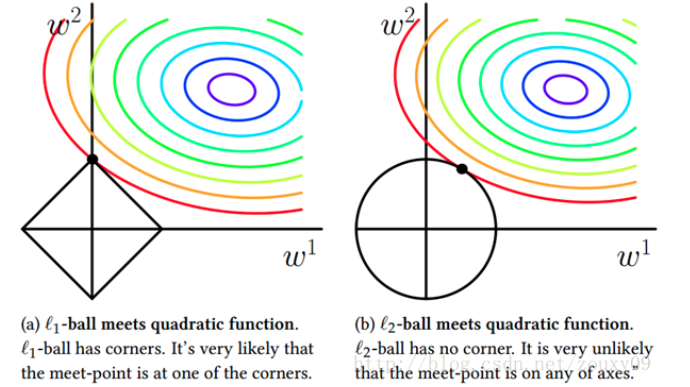
\includegraphics[width=6in]{img/3-2.png}
	\caption{图}\label{fig:3-2}
	\end{figure}
	
	可以看到,在相交的地方,L1在和每个坐标轴相交的地方都有出现解,即更容易出现$w_1$或者$w_2$为0的解,可以用来提取特征,更加容易产生稀疏性。
	
	L2的话更容易出现$w_1$和$w_2$都不是0的情况,虽然有时候会出现很小的值。在更高维的情况下也是这样的,即基本上只是用来正则化而已。
	



\section{数据集增强}

	需要注意的问题
	\begin{itemize}
		\item 不能应用改变正确类别的转换,如:光学字符识别任务需要认识到'b'和'd'的区别,因此对于这种任务来说,水平反转和旋转180度并不是适当的数据集增强方式。
		\item 在神经网络的输入层加入噪声,也可以看成是数据增强的一种形式。然而,神经网络被证明对噪声不是非常健壮。改善神经网络健壮性的方法之一是简单的将随机噪声施加到输入再进行训练。像隐藏单元事假噪声也是可行的,这被看成是在多个抽象层上进行数据集增强。实践证明,噪声被细心调整后,该方法是非常有效的。Dropout可以被看做是通过乘性噪声构建新输入的过程。
		\item 在进行数据集增强的时候,需要进行对照试验。
		
	\end{itemize}
	

\section{提前终止}
	有时候会出现,虽然训练集的误差随着时间的推移逐渐降低,但是训练集的误差再次上升的情况。这种情况下我们需要提前终止模型的训练过程。
	
	提前终止可以单独使用或与其它的正则化策略相结合。
	
	提前终止需要验证集,即这一部分数据相当于在我们的训练过程中是没有参与模型的训练的。我们有两种策略来更好的使用所有的数据。第一种是,第一次训练我们使用训练数据确定最佳的训练步数,然后重新初始化网络,使用所有的数据进行训练。第二种是我们保持从第一轮训练获得的参数,然后使用所有的数据进行训练,但是这样的话,已经没有验证集可以指导我们需要在多少步后进行终止。	
	
\section{参数共享}
	参数共享也是一种正则化方法,是指强迫某些集合中的参数相等。
	
	优点:可以显著减少模型所占用的内存
	
	比如:卷积神经网络
	
\section{bagging}
	Bagging:是通过结合几个模型降低泛化误差的技术。即分别训练几个不同的模型,让所有模型表决测试样例的输出。
	
	Bagging奏效的原因:不同的模型通常不会在测试集上产生完全相同的错误。
	
	假设有k个不同的模型。在不同模型的误差完全相关的情况下,bagging对于降低泛化误差没有任何帮助。但是在模型误差完全不相关的情况下,bagging后的误差仅为之前误差的$\fr\frac{1}{k}$(期望)。这表明,模型的个数越多,则集成模型的误差降低的越小,呈线性关系,即集成后的模型最起码表现的比它的任何一个成员都要好。如果成员之间的误差是独立的,则集成将显著地比其成员表现得更好。
	
	Bagging需要构造k个不同的数据集,每个数据集与原始数据集具有相同数量的样例,但从原始样例中替换采样构成。即新的数据集中包含若干重复的实例,还会缺少很多实例。每个数据集包含样本的差异将导致训练模型之间的差异。
	

\section{Dropout}
	Dropout可以看成是集成非常多的大神经网络的Bagging方法。但是在Dropout中不同的模型之间是共享参数的,也就是说不同的模型之间具有相同的神经元的数量,但是在每一层中的神经元的个数可能是不同的,这一层中使用哪一个神经元也是不同的。
	
	在使用Dropout时,每次训练的过程都只是一个子网络在训练,而不是训练整个网络。这也意味着,在一些小型的神经网路中使用Dropout并不是一个非常好的选择,而应该在一个大型的网络中使用Dropout。也就是说,使用Dropout的代价就是提高了模型的计算代价。需要注意的是,如果你有非常大的训练数据集,使用Dropout进行正则化带来的好处可能小于所带来的计算代价的提升。
	
	同样,在只有极少(如小于5000个)的训练样本可用时,Dropout不会很有效。
	
	Dropout强大的大部分是由于施加到隐藏单元的乘性掩码噪声。BN是在训练时向隐藏单元引入加性和乘性造成,同时这个噪声具有正则化的效果,有时候Dropout变得没有必要。
	
	需要注意的是,在有些深度学习框架中,dropout ratio表示的是保留的神经元的比例,有些是丢弃的神经元的比例。但是在大多数的神经网络的框架中都是表示保留的神经元的比例。
	
\section{Spatial Dropout}
	
	如图所示,对于一个特征来说,传统的Dropout在随机丢弃点的时候,会丢弃这个特征中的一些点。而Spatial Dropout会直接丢弃整个特征。在实际的应用中,如在做物体检测,或者使用Unet的过程中Spatial Dropout的表现是更好的。
	\begin{figure}[!htbp]
	\centering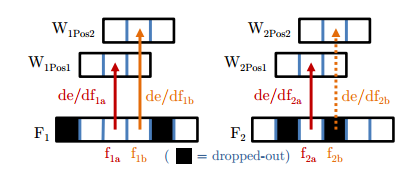
\includegraphics[width=6in]{img/3-3.png}
	\caption{原始Dropout}\label{fig:3-3}
	\end{figure}
	\newpage
	
	\begin{figure}[!htbp]
	\centering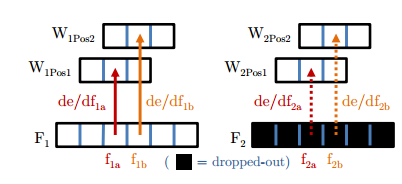
\includegraphics[width=6in]{img/3-4.png}
	\caption{Spatial Dropout}\label{fig:3-4}
	\end{figure}

\section{对抗训练}

	\begin{figure}[!htbp]
	\centering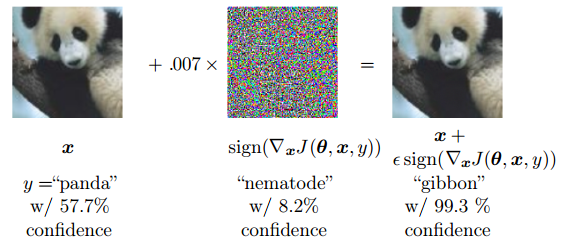
\includegraphics[width=6in]{img/3-5.png}
	\caption{图}\label{fig:3-5}
	\end{figure}
	
	通过添加一个不可察觉的小向量,我们可以改变GoogleNet对此图像的分类结果。如上图所示,我们人类可能不能观察出这种区别,但是网络的预测结果可能会千差万别。
	
	对于上述这种情况我们可能需要使用对抗训练来进行正则化。
	
	但是具体对抗训练是什么样的,暂时不清楚。---待补充
	
	
	
	
	
	
	
	
	
	
	
	
	
	
	
	
	
	
	
	
	
	
\cleardoublepage
%第四章 优化方法
\chapter{训练优化方法}

\section*{Introduction}
	本章节内容主要介绍深度学习中遇到的优化方法
	
	
	
	
	
	
	
	
	
	
	
	
	
	
	
	
	
\cleardoublepage
%第五章 一些传统的机器学习方法
\chapter{机器学习}

\section*{Introduction}
	本章节主要介绍一些常用的机器学习方法,部分内容参考《统计学习方法》李航
	

\section{决策树}
	
	\subsection{熵}
	熵,表示一个信号源发出的信号的不确定程度。在信源发出的信号中,某信号出现的概率越大,熵越小。熵只依赖于分布,而与具体的取值无关。如果用随机变量来表示的话,熵越大,表示随机变量的不确定性越大。
	
	香农使用log函数来定义样本i的信息熵:
	
	\begin{equation}
		f(p(i)) = \log \frac{1}{p(i)} = -\log p(i)
	\end{equation}
	
	因此在有n个样本的时候,我们用如下的公式来表示所有样本集合的信息熵:
	
	\begin{equation}
		E(P) = \sum_{i}^{n} \log p(i) \frac{1}{p(i)} = -\sum_{i}^{n} p(i)\log p(i)}
	\end{equation}
	
	然而,在机器学习中,我们通常使用模型分布q(i)来逼近真实分布p(i),因此交叉熵的公式为:
	
	\begin{equation}
		E(P,Q) = -\sum_{i}^{n} p(i)\log q(i)}
	\end{equation}
	
	在tensorflow或者其他的深度学习框架中,我们使用的也是如上的公式来表示交叉熵。y表示网络的输出,y\_ 表示真是的label,公式如下:
	
	\begin{equation}
		cross\_entropy = -\sum_{i}^{n} y\_\log y}
	\end{equation}
	
	\subsection{信息增益}
	
	我们使用g(D,A)来表示特征A对数据集D的信息增益,E(D)表示数据集D的熵,E(D|A)表示在给定特征A的条件下D的经验熵。那么,我们可以使用如下的公式来表示信息增益:
	
	\begin{equation}
		g(D,A) = E(D) - E(D|A)
	\end{equation}
	
	E(D)表示对数据集D进行分类的不确定性,E(D|A)表示在给定特征A下对D分类的不确定性,那么它们的差就表示在使用了特征A后数据集信息不确定性的减少的程度。
	
	信息增益的大小是相对于数据集而言的,并没有绝对意义,因此信息增益比可以解决这个问题。信息增益比:
	
	\begin{equation}
		g_{R}(D,A) = \frac{g(D,A)}{E(D)}
	\end{equation}
	
	在具体的算法中如果需要计算信息增益或者信息增益比,只需要分别计算E(D),E(D|A)即可。计算$p_i$时只需要计算$C_i$这一类在整个数据集中出现的次数即可,其他相关的参数也是类似计算。
	
	\subsection{决策树生成}
	
	\subsubsection{ID3}
		对于训练数据D,特征集A,阈值$\epsilon$
		\begin{itemize}
			\item 如果D中的所有实例都属于同一类,则为一棵单节点树,算法结束。
			\item 如果特征集A为空,则T为单节点数,选择实例中出现次数最多的类作为该节点的类标记,算法结束
			\item 如果上述两条不满足,计算所有特征的信息增益,并选择信息增益最大的特征$A_k$,如果$A_k$小于阈值,则为单节点树,选择实例中出现次数最多的类作为该节点的类标记,算法结束。否则,对于$A_k$的每一个可能值$a_i$,对数据集D进行划分,这个划分就是这棵树的多个子树。
			\item 重复上述步骤即可得到一颗决策树。
		\end{itemize}
	\subsubsection{C4.5}
	C4.5算法与ID3的不同之处是使用信息增益比来进行特征的选择。
	
	\subsection{防止过拟合}
	
	决策树的生成过程只考虑局部最优,这样就会造成全局不是最优的结果。因此,剪枝的过程中需要考虑全局最优。
	
	决策树的剪枝通过最小化决策树的整体损失函数来实现。设决策树T有|T|个节点,t为树T的叶节点,该叶节点有$N_t$个样本点,其中属于k类的样本点有$N_{tk}$个,$E_t(T)$为叶节点的熵,$\alpha$为正则化参数,则决策树的损失函数定义为:
	
	\begin{equation}
	L = \sum _{t=1} ^{|T|}N_t E_t(T) + \alpha |T|
	\end{equation}
	
	决策树的损失函数表示的意思为,在保证整个数据集中样本点的熵的和尽量小的前提下,使得决策树中节点的数量更小。也就是说对于一些叶节点中样本的数量较少的节点,我们直接向上收缩,将这一个叶节点直接减掉,将其归到前一个分类条件中去。
	
	\subsection{CART算法}
	\subsubsection{回归树}
	\subsubsection{分类树}
	
\section{随机森林}
	随机森林在属性(列)和数据(行)的使用上进行随机化,生成许多分类树,再汇总分类树的结果。随机森林在运算量没有显著提高的基础上提高了精度。
	
	每棵决策树都只对部分数据进行决策,而随机采样可以保证有重复的样本被不同的决策树所分类,这样就可以对决策树的分类能力做出评价。
	
	随机森林与Bagging有些类似。以决策树为基本模型的bagging在每次bootstrap放回抽样后,产生一次决策树,抽多少样本就产生多少棵树,在生成这些树的时候没有进行过多的干预。随机森林也是基于bootstrap进行随机抽样,但是每个节点的变量都是在随机产生的变量中产生。因此,不但样本是随机的,连每个节点变量的产生都是随机的。
	
	随机森林的loss function:熵
	
	\subsection{算法过程}
	\begin{itemize}
		\item 首先是两个随机采样。对于每一棵决策树来说,都需要对行进行随机选择(有放回,可能会产生重复样本),然后进行列采样,即从所有的特征中抽取部分特征。这样每棵树所使用的数据都不是所有的数据。这两个随机性的加入使得随机森林不至于过拟合。(首先进行行采样,然后在每个节点分裂成子树的时候随机选择列,再计算信息增益等信息进行特征选择)
		\item 然后对对于每一棵决策树来说,都采用完全分裂的方式建立。建立的过程同上一节的内容
		\item 由于步骤一的两个随机性的加入,使得随机森利即使不进行剪枝也不会出现过拟合的现象。
		\item 将生成的多棵决策树组合成随机森林,用随机森林分类器对新的数据进行判别与分类。分类结果按照多数表决决定。
	\end{itemize}
	
	
	\subsection{算法优缺点}
	\subsubsection{优点}
	\begin{itemize}
		\item 两个随机性的引入,使得随机森林不容易过拟合,同时抗噪声能力更强
		\item 在处理高维数据的时候,不需要进行特征选择。顺便还可以确定重要的变量。
		\item 对数据的适应能力强,既能处理离散数据又能处理连续数据,数据集不需要进行规范化,不需要预处理,对缺失数据,非平衡数据稳健。
		\item 训练速度快,可以得到变量重要性的排序。可以进行特征提取
		\item 简单调参即可,跑一组试验画个图即可决定树的棵树。
	\end{itemize}
	\subsubsection{缺点}
	\begin{itemize}
		\item 模型规模大,评估速度慢
		\item 难以解释清楚
	\end{itemize}
	
	

	
	
	
\section{GBDT}	
	GBDT(Gradient Boosting Decision Tree),是一种迭代决策树算法。该算大由多棵决策树组成,所有树的结论累加起来作为最终答案。
	
	\subsection{回归树}
	随机森林中的树都是分类树,主要用于处理分类的情况。GBDT中的树都是回归树,搞清楚这一点是非常重要的。
	
	
	\subsection{一些注意事项}
	\begin{itemize}
		\item 自动发现有效的特征,特征组合,用来作为LR中的特征
		\item 每个节点得到一个预测值,最小化平方误差
		\item 以CART作为基分类器,基尼系数越大,不确定性越高$Gini(D,A) = \frac{|D_1|}{|D|} Gini(D_1)+ \frac{|D_2|}{|D|} Gini(D_2) $
	\end{itemize}	



\section{支持向量机}
	\subsection*{Introduction}
	SVM的决策函数为$sign(wx+b)$
	
	\subsection{预备知识}
		\subsubsection{函数间隔}
		在SVM中,分类的决策边界为一个超平面$wx+b=0$,一般来说,一个点距离这个超平面的远近可以表示分类的确信程度,在超平面确定的情况下,$|wx+b|$可以表示点到超平面的距离。而$wx+b$的符号可以表示分类正确与否,即是否与y一致。因此,可以使用$y(wx+b)$用来表示分类的正确性与确定度,这就是函数间隔:
		
		\begin{equation}
			\hat{\gamma_i} = y_i(wx_i+b)
		\end{equation}
		
		但是函数间隔存在的一个致命的问题就是,当我们等比例的改变w和b的时候,函数间隔也在等比例的改变,但是此时我们用来分类的超平面却没有改变。这样当我们最大化间隔的时候将没有任何意义,因此我们需要对超平买你的法向量做一些约束,比如对w进行规范化,$\|w\|=1$,使得对于一个超平面来说,间隔是确定的,这样就成了几何间隔。
		
		\subsubsection{几何间隔}
		如上所述,我们可以得到几何间隔的定义。对于给定的数据集T,给定的超平面$wx+b=0$,样本点$(x_i,y_i)$到超平面的几何间隔为:
		
		\begin{equation}
			\gamma_i = y_i(\frac{w}{\|w\|})x_i + \frac{b}{\|w\|}
		\end{equation}
		
		由于我们在使用SVM的时候最有是要取最大的间隔,以上为每个点的几何间隔,因此我们需要得到所有点的几个间隔的最小值($\gamma = \min \gamma_i $),我们只要使得这个最小值最大化,就可以获得我们的最终结果。$\gamma$为整个数据集的几何间隔,$\gamma_i$为第i个数据的几何间隔。
		
		从函数间隔和几何间隔的定义我们可以得到它们之间的关系,如下式所示,当$\|w\|=1$的时候,函数间隔和几何间隔是相等的,但是如果等比例的改变w和b,函数间隔等比例的改变,但是几何间隔不变。
		
		\begin{equation}
		\gamma = \frac{\hat{\gamma}}{\|w\|}
		\end{equation}
	\subsection{硬间隔最大化}
	我们的主要目的是获得一个分类平面,并且使得所有数据到这个平面的距离尽可能的远。即最大化几何间隔,使得数据集中的每个样本点到超平面的几何间隔最小是$\gamma$
	
	\begin{equation}
		\max_{w,b}\ \gamma
	\end{equation}
	
	\begin{equation}
		s.t.\ y_i(\frac{w}{\|w\|}x_i + \frac{b}{\|w\|}) \geq \gamma
	\end{equation}
	
	根据函数间隔与几何间隔的关系我们可以将上述公式转化为下面的公式:
	
	\begin{equation}
		\max_{w,b}\ \frac{\hat{\gamma}}{\|w\|}
	\end{equation}
	
	\begin{equation}
		s.t.\ y_i(wx_i+b) \geq \hat{\gamma}
	\end{equation}
	
	对于上面的公式来说,即使等比例的改变w和b,也不会对目标函数的优化造成影响,因为等比例改变w和b,虽然目标函数等比例的改变了,约束条件也会因此改变。也就是说,上式中函数间隔其实对结果没有任何作用。因此,我们可以使函数间隔为一个固定的值,在这里我们使$\hat{\gamma} = 1$,这样上述公式就简化了,同时我们将最大化问题改成最小化问题,就得到了下面的最优化问题。硬间隔最大化的SVM公式如下:
		
	\begin{equation}
		\min_{w,b}\ \frac{1}{2}\|w\|^{2}
	\end{equation}
	
	\begin{equation}
		s.t.\ y_i(wx_i+b) -1 \geq 0
	\end{equation}
	
	求解上述公式可以得到$w^*,b^*$,这样进一步我们就可以得到SVM分类的决策函数$f(x) = sign(w^*x+b^*)$
	
	\subsection{硬间隔最大化的对偶问题}
	通过求解对偶问题可以得到原始问题的解,(最优化中的对偶问题,本章不做详细的描述),这样做有两个有点,一方面是对偶问题往往更容易求解,一方面是自然的引入了核函数。
	
	首先我们需要构造拉格朗日函数,引入拉格朗日乘子$\alpha_i \geq 0$,定义拉格朗日函数为:
	
	\begin{equation}
	L(w,b,\alpha) = \frac{1}{2}\|w\|^2-\sum_{i=1}^{N}\alpha_i(1-y_i(wx_i+b))
	\end{equation}
	
	现在问题等价于求解$\min_{w,b}\ \max_{\alpha} L(w,b,\alpha)$,等价于求解$\max_{\alpha} \ \min_{w,b} L(w,b,\alpha)$,那么我们首先需要求解$\min_{w,b} L(w,b,\alpha)$,求解这个式子需要令其对于w和b的偏导数等与0,即:
	
	\begin{equation}
		\frac{\partial_L}{\partial_w}=\|w\| - \sum x_i y_i = 0
	\end{equation}

	\begin{equation}
		\frac{\partial_L}{\partial_b}=\sum \alpha_i y_i = 0
	\end{equation}
	
	将上面的导数带回原式得到:
	
	\begin{equation}
	L(w,b,\alpha) = -\frac{1}{2}\|w\|^2 + \sum_{i=0}^{N} \alpha_i
	\end{equation}
	
	接下来只需要求$\max_{\alpha}L(w,b,\alpha)$,取负号即可直接转换成最小化问题,得到新的函数为:

    \begin{equation}
	\min_{\alpha} \frac{1}{2}\|w\|^2 - \sum_{i=0}^{N} \alpha_i
	\end{equation}
	
	\begin{equation}
	s.t.\ \sum_{i=1}^{N} \alpha_i y_i = 0
	\end{equation}
	
	\begin{equation}
	\qquad \alpha_i \geq 0, \ i=1,2,...N
	\end{equation}
	
	可以根据上述三个公式求得$\alpha^*$,然后进一步求得$w^*,b^*$,最终求得原始问题的解。下面还有一个问题就是,我们求得的解究竟是不是原始问题的解,如果是的话需要满足如下的KKT条件:
	
	\begin{equation}
		\frac{\partial_L(w^*,b^*,\alpha^*)}{\partial_w} = 0
	\end{equation}

	\begin{equation}
		\frac{\partial_L(w^*,b^*,\alpha^*)}{\partial_b} = 0
	\end{equation}
	
	\begin{equation}
		\alpha_i^*(y_i(w^*x_i+b^*)-1)=0,i=1,2,...,N
	\end{equation}
	
	\begin{equation}
		y_i(w^*x_i+b^*)-1 \geq 0,i=1,2,...,N
	\end{equation}
	
	\begin{equation}
		\alpha_i^* \geq 0,i=1,2,...,N
	\end{equation}
	
	



\section{AdaBoost}
	本章内容来自于网络以及张志华老师的就《机器学习导论》课程

	本章基本内容就是给定一堆弱分类器,然后通过各种组合组成一个人强的分类器
	\subsection{离散的AdaBoost}
	离散的AdaBoost算法步骤:\boldmath  %公式加粗

	$w$表示给数据的权值,$\alpha$表示给分类器的权值

	\begin{enumerate}		
		\item start with weights $w_i = \frac{1}{N} \quad i=1...N$
		\item repeat for m=1 to M
			\begin{itemize}
				\item 使用输入数据训练一个分类器$G_m(x) \in (-1,1)$
				\item 计算误差err:
					\begin{equation*}
						E_w[I_(y_i\not \equiv G_m(x_i))]=\frac{\sum_{i=1}^{N}w_i I_(y_i\not \equiv G_m(x_i))}{\sum_{i=1}^{N}w_i}
					\end{equation*}
				\item 输出$\alpha_m = \frac{1}{2}log(\frac{1-err}{err})$,从这里可以看出分类器的误差越大,权值越小
				\item set $w_i = \frac{w_i}{Z_m} \exp(\alpha_m I_(y\not \equiv G_m(x))$,其中$Z_m$是规范化因子,\newline
				$Z_m=\sum_{i=1}^{N}w_i \exp(-\alpha_m y_i G_m(x_i))$如果一个数据点分类错了,那么给这个点的权值大一点。
			\end{itemize}
		\item 这样我们就得到了$G(x)=sign[\sum_{m=1}^{M}\alpha_m G_m(x)]$
	\end{enumerate}
	
	
	\subsection{Forward Stagest Additive Modeling}

	考虑加法模型(additive model)\boldmath
	\begin{equation}
		f(x)=\sum_{m=1}^{M}\beta_{m}b(x;\gamma_{m})
	\end{equation}
	其中,$b(x;\gamma_{m})$为基函数,$\gamma_m$为基函数的参数,$\beta_m$为基函数的系数。

	在给定训练数据以及Loss Function的情况下,相当于一个加法模型$f(x)$相当于一个minimize Loss Function的问题:
	\begin{equation}
		min_{\beta_m,\gamma_m} \sum_{i=1}^{N}L(y_i,\sum_{m=1}^{M}\beta_{m}b(x;\gamma_{m}))
	\end{equation}
	从前向后,每一步值学习一个基函数及其系数,即每一步只需优化如下的损失函数:
	\begin{equation}
		min_{\beta,\gamma} \sum_{i=1}^{N}L(y_i,\sum_{m=1}^{M}\beta b(x;\gamma))
	\end{equation}
	\newline
	\newline

	前向分布算法:

	输入:训练数据$T={(x_1,y_1),...(x_N,y_N)}$,Loss Function$L(x,f(x))$,基函数$b(x;\gamma)$

	输出:加法模型$f(x)$

	\begin{enumerate}		
		\item 初始化$f_0(x)=0$
		\item repeat for m=1 to M
			\begin{itemize}
				\item 计算参数$\beta_m,\gamma_m$
				\begin{equation}
					(\beta_m,\gamma_m)=\arg\min_{\beta,\gamma} \sum_{i=1}^{N}L(y_i,f_{m-1}(x_i)\beta b(x;\gamma))
				\end{equation}
				\item 更新$f_m(x)=f_{m-1}(x)+\beta_m b(x;\gamma_m)$
			\end{itemize}
		\item 得到加法模型
				\begin{equation}
					f(x)=\sum_{m=1}^{M} \beta_m b(x;\gamma_m)
				\end{equation}
	\end{enumerate}
	
	


\cleardoublepage 
\chapter{Deep Learing}

\section*{Introduction}
	本章节内容主要是来自于深度学习中遇到的一些坑以及问题
	
\section{一些小的trick}

1. 一定要对数据进行归一化

2. 训练可能会出现loss一开始迅速下降,然后稳定在一定的值上,这时候不要以为网络已经收敛了,有时候会出现一个拐点,即在训练很后面的时候会重新出现一个新的下降的区间,这时候网络基本上会收敛。但是不排除会出现多的拐点的情况。结论:训练过程中一定要耐心耐心再耐心。
	
\section{weight decay}
	\boldmath  %公式加粗
	在损失函数中,weight decay是放在正则项(regularization)前面的一个系数,正则项一般指示模型的复杂度,所以weight decay的作用是调节模型复杂度对损失函数的影响,若weight decay很大,则复杂的模型损失函数的值也就大。我所理解的weight decay就是一个调节正则化项的系数,增大则对正则化项的依赖会更高,不容易过拟合,反之则反之。
	
	利用weight decay给损失函数加了个惩罚项,使得在常规损失函数值相同的情况下,学习算法更倾向于选择更简单(即权值和更小)的NN。是一种减小训练过拟合的方法。
	
	Weight decay is equivalent to L2 regularizer.
	
	在训练神经网络的时候,可以先设置weight decay为0,然后使网络过拟合,查看测试结果。结果正确后,设置weight decay为大一点的值,即加入正则化项,这样可以防止过拟合现象。具体大小需要在网络中调试。
	
	遇到的问题:在训练U-net的时候,出现训练结果全是黑图的情况。原因是weight decay设置过大,导致网络结果没有过拟合。解决方案:设置weight decay为更小的值。
	

\section{momentum}
	momentum是梯度下降法中一种常用的加速技术。对于一般的SGD,其表达式为$x \gets x-\alpha * dx$,x沿负梯度下降。而带momentum项的SGD则写生如下形式:$v=  \beta *v -a*dx$,$x \gets x+v$,其中$\beta$是momentum系数,通俗的理解上面式子就是,如果上一次的momentum(即v)与这一次的负梯度方向是相同的,那这次下降的幅度就会加大,所以这样做能够达到加速收敛的过程。
	
	神经网络的训练过程(也就是梯度下降法)是在高维曲面上寻找全局最优解的过程(也就是寻找波谷),每经过一次训练epoch,搜寻点应该更加靠近最优点所在的区域范围,这时进行权重衰减便有利于将搜寻范围限制在该范围内,而不至于跳出这个搜索圈,反复进行权重衰减便逐渐缩小搜索范围,最终找到全局最优解对应的点,网络收敛。momentum是冲量单元,也就是下式中的m,作用是有助于训练过程中逃离局部最小值,使网络能够更快速地收敛,也是需要经过反复地trial and error获得的经验值
	
	主要作用:防止陷入局部最小值


\cleardoublepage 
\chapter{Caffe}

\section*{Introduction}
	本章节内容主要是关于caffe框架的一些知识。
	

\section{lmdb}
	lmdb格式的文件在使用Python程序进行生成的时候,如果需要重复生成,则需要先删除原来的。否则会在原先的lmdb上重新添加文件。


	
\section{net protobuf}
	\boldmath  %公式加粗
	此部分内容有待添加
	
	

\section{solver}	
	solver文件为caffe的训练参数的文件,主要存储一些训练的超参数
    
    运行代码为:# caffe train --solver=*slover.prototxt
    
    一个例子:
    
    \begin{lstlisting}
    train_net: "lenet_train.prototxt"
    test_net: "lenet_test.prototxt"	
	test_iter: 100
	test_interval: 500
	
	base_lr: 0.01
	lr_policy: "fixed"
	
	momentum: 0.9
	type: SGD
	weight_decay: 0.0005
	display: 100
	max_iter: 20000
	snapshot: 5000
	snapshot_prefix: "models"
	solver_mode: CPU
	\end{lstlisting}
	
	下面来一个一个解释这些程序的意思
    
    1.    
        
    train\_ net: "lenet\_ train.prototxt"
    
    test\_ net: "lenet\_ test.prototxt"
    	
    这两行用于定于训练网络和测试网络,可以是同一个网络,用net:train\_ test.prototxt 来表示,为上一节的内容。注意:文件的路径要从caffe的根目录开始,其他所有的配置都是这样的。
    
    2.接下来test\_ iter 表示一次训练需要加载多少个数据,许训练中的batch size是一致的;test\_ iterval表示经过多少此训练的Iteration后进行一次测试,如500表示没经过500个Iteration进行一次测试。另外,如果网络不想进行测试的话,可以在solver文件中加入如下的参数 test\_ initialization: false 这样不管经过多少次的Iteration都不会进行测试。
    
    3.有关于learing rate的东西
    
    base\_ lr 表示初始的一个learing rate,如果lr\_ policy 如果设置为fixed,训练过程中会一直维持这个learing rate不再改变,其他的都是会在训练过程中逐渐变化的。
    
    lr\_ policy 可设置的值如下所示:
    \begin{itemize}
    	\item fixed:保持base\_ lr不变
    	\item step: 如果设置为step,则还需要设置一个stepsize,返回 $base\_ lr*gamma^{floor*         \frac{iter}{stepsize}}$,其中iter表示当前的迭代次数。如设置gamma=0.9,stepsize=100表示在第一百次迭代后learning rate 下降到原来的0.9倍
    	\item exp:返回$base\_ lr * gamma ^ iter$, iter为当前迭代次数
    	\item inv:如果设置为inv,还需要设置一个power, 返回$base_lr * (1 + gamma * iter) ^ {- power}$
    	\item multistep:如果设置为multistep,则还需要设置一个stepvalue。这个参数和step很相似,step是均匀等间隔变化,而multistep则是根据stepvalue值变化
    	\item poly:学习率进行多项式误差, 返回 $base\_lr (1 - iter/max\_ iter) ^ {power}$
    	\item sigmoid:学习率进行sigmod衰减,返回 $base\_lr ( 1/(1 + exp(-gamma * (iter - stepsize))))$
    
    \end{itemize}
    需要设置参数的数量随着lr pilicy的不同而有所变化。如设置为fixed则不需要添加任何参数,设置为step则需要添加gamma和stepsize两个参数,设置为step的策略后solver配置如下所示:
    \begin{lstlisting}
	base_lr: 0.01
	lr_policy: "step"
	gamma:0.9
	stepsize:100
	\end{lstlisting}
	
	4.对于momentum,一般取值在0.5--0.99之间。通常设为0.9,momentum可以让使用SGD的深度学习方法更加稳定以及快速。详细的资料,参考Hinton的论文《A Practical Guide to Training Restricted Boltzmann Machines》
    
    5. type:SGD
    
    表示优化算法,总共有六种:SGD、AdaDelta、AdaGrad、Adam、NAG、RMSprop
    
    6.weight\_ decay 为权重衰减项,详细的内容已经在上一章解释过了。
    
    7.display:100表示没训练100个Iteration显示一次loss
    
    8.max\_ iter:2000 表示最大的迭代此时为2000
    
    9.
    
    snapshot:500
    
    snapshot\_ prefix :"models" 
    
    表示没训练500个Iteration,保存一次网络的参数数据,保存路径为models。同时会保存另外一个solverstate文件,以便下次训练的时候可以从这一步继续训练。
    
    10.solver\_ mode: CPU设置运行模式为CPU




\section{一些其他的问题}
	\subsection{loss=87.3365}
		\begin{itemize}
			\item 如果一开始就出现这种情况,有可能是参数的初始化方式不对,使用xavier可以避免这种情况
			\item 在caffe中数据的标签必须从0开始,且为整数(1.0,2.0也可以)
			\item 数据可能会出现问题(一定要反复确定数据没有问题才可以)
			\item 如果是图片数据可能是图片没有进行归一化,最好是进行归一化并且减去均值
			\item 如果一开始的loss是在下降的,但是训练到后期出现了87.3365这个值,代表网络发散了,需要调整learing rate到一个较小的值,建议从0.01开始,到0.0001即可适合大部分网络结构
		\end{itemize}
		
	\subsection{一些差别}
		solver.step(1) 表示网络进行一次迭代,即进行一次前向过程和一次反向传播
		
		solver.net.forward() 表示网络只进行一次前向的过程,可用于网络的预测
		
	\subsection{多GPU计算}
		如果使用solver文件:build/tools/caffe train --solver=models/bvlc\_ alexnet/solver.prototxt --gpu=0,1
		
		如果使用Python文件:python yourpythonfile.py CUDA\_ VISIBLE\_ DEVICES=0, 1
	




	% \begin{enumerate}		
	% 	\item start with weights $w_i = \frac{1}{N} \quad i=1...N$
	% 	\item repeat for m=1 to M
	% 		\begin{itemize}
	% 			\item 使用输入数据训练一个分类器$G_m(x) \in (-1,1)$
	% 			\item 计算误差err:
	% 				\begin{equation*}
	% 					E_w[I_(y_i\not \equiv G_m(x_i))]=\frac{\sum_{i=1}^{N}w_i I_(y_i\not \equiv G_m(x_i))}{\sum_{i=1}^{N}w_i}
	% 				\end{equation*}
	% 			\item 输出$\alpha_m = \frac{1}{2}log(\frac{1-err}{err})$,从这里可以看出分类器的误差越大,权值越小
	% 			\item set $w_i = \frac{w_i}{Z_m} \exp(\alpha_m I_(y\not \equiv G_m(x))$,其中$Z_m$是规范化因子,\newline
	% 			$Z_m=\sum_{i=1}^{N}w_i \exp(-\alpha_m y_i G_m(x_i))$如果一个数据点分类错了,那么给这个点的权值大一点。
	% 		\end{itemize}
	% 	\item 这样我们就得到了$G(x)=sign[\sum_{m=1}^{M}\alpha_m G_m(x)]$
	% \end{enumerate}



%--------------------------------------------------------------------------------
%--------------------------------------------------------------------------------
%--------------------------------------------------------------------------------
\cleardoublepage 


\renewcommand{\refname}{Reference} % Change the default bibliography title

\bibliography{sample} % Input your bibliography file

%----------------------------------------------------------------------------------------

\end{document}